% !TeX root = ../FoodSpy.tex
% \section{Framework-uri web}

\section{Angular}
Numele ”Angular” vine de la caracterele ”<” și ”>” (în engleză, ”angled brackets”) care delimitează numele tuturor tag-urilor din HTML, de exemplu ”<a>” sau ”<div>”.
Angular este o platformă de dezvoltare, bazată pe limbajul TypeScript, care este un superset al limbajului JavaScript. Angular este un framework care face posibilă implementarea într-un mod trivial a cerințelor complexe ale aplicațiilor web, cum ar fi animații sau ”data binding”.
\\ \\
Platforma Angular oferă un mod de lucru bazat pe componente individuale care duce cu ușurință la construirea de aplicații web scalabile, dar și la posibilitatea reutilizării acestor componente în alte aplicații.
Angular vine integrat cu o multitudine de biblioteci care acoperă o gamă largă de cazuri de utilizare, printre care comunicarea cu un server și validarea formularelor HTML (Fig. \ref{fig:41}).

\begin{figure}[!htb]
	\centering
	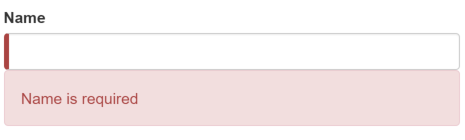
\includegraphics[width=0.5\textwidth]
	{../LaTeX/Images/angular_hero-form-2.PNG}
	\caption{Validarea câmpului ”Name” din formular}
	\label{fig:41}
\end{figure}

Mai mult, Angular este gândit să faciliteze actualizarea cât mai ușoară a aplicației, de aceea pune la dispoziție o suită de unelte care ajută la dezvoltarea, testarea și actualizarea codului printre care și ”Live Reload”, o funcționalitate prin care aplicația web este recompilată și deservită la orice modificare a codului-sursă.

\subsection{Components}
Asemenea blocurilor de LEGO, componentele Angular sunt puse laolaltă pentru a construi o aplicație web. O componentă (Fig. \ref{fig:42}) este formată dintr-o clasă TypeScript, adnotată cu decoratorul ”@Component”, un șablon HTML și opțiuni de stilizare.
\\ \\
În clasa TypeScript este scris codul care determină funcționalitatea componentei, șablonul HTML spune cum este structurată componenta, iar opțiunile de stilizare definesc aspectul acesteia. Această separare ajută la testarea mai ușoară a codului și lizibilitatea acestuia.

\begin{figure}[!htb]
	\centering
	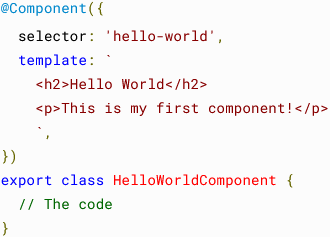
\includegraphics
	{../LaTeX/Images/angular_components.PNG}
	\caption{O componentă Angular}
	\label{fig:42}
\end{figure}

Componenta se folosește printr-un apel după numele descris sub proprietatea ”selector”, în cazul acesta ”<hello-world></hello-world>”.

\subsection{Templates}
”Template” sau ”șablonul” descrie felul în care este structurată componenta folosind limbaj HTML. Limbajul HTML poate fi scris ”inline”, cum se vede în (Fig. \ref{fig:42}) sub proprietatea ”template” sau poate fi scris într-un fișier separat cu extensia ”.html”.
Angular extinde capabilitățile limbajului HTML oferind așa numitele ”directives”, care sunt clase ce pot modifica în mod dinamic structura aplicației.
\\ \\
De exemplu, ”*ngIf” poate fi folosit pe un ”<div>” (dar și alte tag-uri HTML) pentru a-l afișa sau nu în funcție de valoarea unei variabile de tip ”boolean”, astfel:

\begin{verbatim}
	<div *ngIf=”showDiv”>
	<p> Dacă ”showDiv” este ”true” atunci ”<div>” este vizibil în pagină </p>
	</div>
	
	<div *ngIf=”!showDiv”>
	<p> Dacă ”showDiv” este ”false” atunci ”<div>” nu este vizibil în pagină </p>
	</div>
\end{verbatim}

De reținut este faptul că ”showDiv” este o variabilă ce a fost definită în clasa TypeScript a componentei.

\subsection{Dependency Injection}
Prin ”dependency injection” a se înțelege un design pattern prin care este posibilă scrierea de cod-sursă mai flexibil și mai ușor de testat. În Angular, prin ”dependency injection”, într-o clasă se pot declara dependințe către alte clase, fără să fie necesară instanțierea explicită a lor - instanțierea se efectuează în mod automat.
O clasă către care este definită o dependință din altă clasă trebuie să fie adnotată cu decoratorul ”@Injectable”, astfel:

\begin{figure}[!htb]
	\centering
	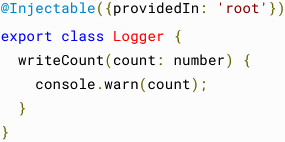
\includegraphics
	{../LaTeX/Images/angular_injectable.PNG}
	\caption{”Logger” este o clasă ce poate fi ”injectată”}
	\label{fig:44}
\end{figure}

Funcția ”writeCount()” din clasa ”Logger” este folosită mai departe în interiorul clasei ”HelloWorldDependencyInjectionComponent”, după cum se vede în (Fig. \ref{fig:45}).

\begin{figure}[!htb]
	\centering
	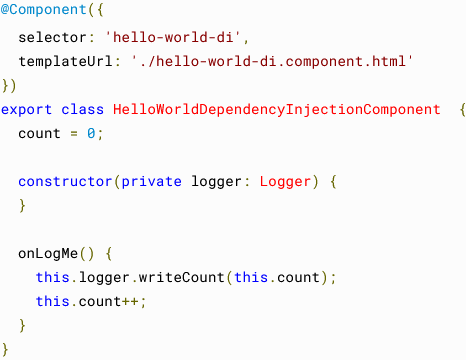
\includegraphics
	{../LaTeX/Images/angular_dependency-injection.PNG}
	\caption{”HelloWorldDependencyInjectionComponent” cu membrul ”private logger”}
	\label{fig:45}
\end{figure}

A se observa constructorul clasei ”HelloWorldDependencyInjectionComponent”, unde s-a definit o dependință către clasa ”Logger” prin membrul ”private logger”.

\section{ASP.NET Core}
ASP.NET Core este un framework web, care rulează pe platforma .NET și .NET Core. Bazat pe limbajul de programare C\#, ASP.NET Core suportă construirea serviciilor REST (așa numitele API-uri web).
Un ”request” sau o ”cerere” venită către un asemenea serviciu REST este tratată de către un controller. În ASP.NET Core, un controller este o clasă ce derivă din clasa de bază ”ControllerBase”.

\begin{figure}[!htb]
	\centering
	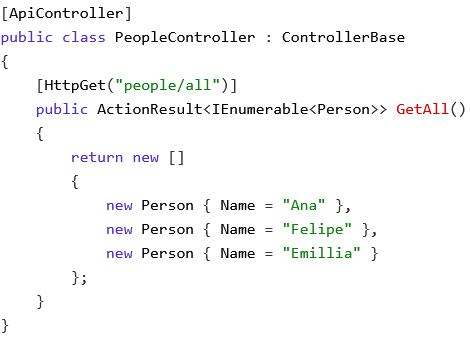
\includegraphics[width=0.8\textwidth]
	{../LaTeX/Images/asp_controller-1.PNG}
	\caption{”PeopleController” este un exemplu de controller}
	\label{fig:46}
\end{figure}

Deoarece ”PeopleController” este adnotat cu atributul ”[HttpGet("people/all")]”, acesta este capabil să răspundă cererilor metodei ”GET” efectuate la URL-ul ”/people/all”.
\\ \\
”people/all” se mai numește ”endpoint” și intrinsec este configurat să răspundă într-un mod serializabil, sub forma unui JSON, după cum se poate observa în (Fig. \ref{fig:47}).

\begin{figure}[!htb]
	\centering
	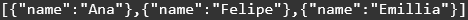
\includegraphics
	{../LaTeX/Images/asp_response.PNG}
	\caption{Exemplu de răspuns dat de un controller}
	\label{fig:47}
\end{figure}

După cum se poate observa și în exemplele de mai sus, ASP.NET Core permite definirea ”inline” a endpoint-urilor și metodelor REST prin adnotări, folosind atribute.
Un exemplu de controller capabil să răspundă la metodele ”GET” și ”POST” este ilustrat în (Fig. \ref{fig:48}).

\begin{figure}[!htb]
	\centering
	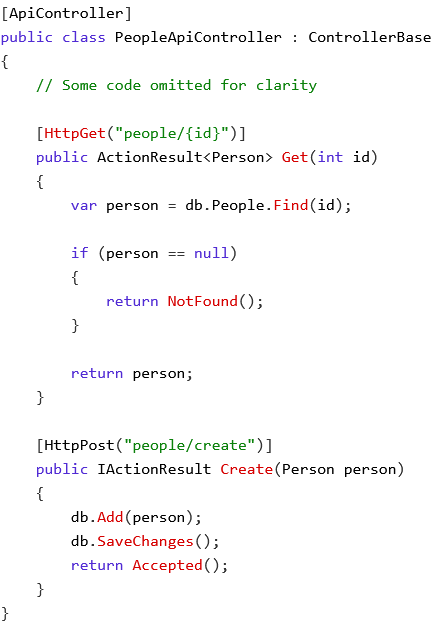
\includegraphics[width=0.6\textwidth]
	{../LaTeX/Images/asp_controller-2.PNG}
	\caption{Exemplu controller}
	\label{fig:48}
\end{figure}

În practică deci, un web API construit folosind ASP.NET Core nu este altceva decât o colecție de unul sau mai multe controller-e care sunt capabile să răspundă cererilor venite din partea interfeței-utilizator (și nu numai).